\documentclass[UTF8]{article}
\usepackage{ctex}
\usepackage{amsmath}
\usepackage{amssymb}
\usepackage{listings}
\usepackage{graphicx}

\usepackage{caption}
\begin{document}
% 词向量 部分 begin
\paragraph{\large 3.2.4 lstm词向量}
 \subparagraph{}词向量是NLP中最基本的概念之一,词向量将抽象的语言符号化数学化。主要分为两种:
 \subparagraph{one-hot representation:\\}


    举个例子:\\
    “话筒”表示为 [0 0 0 1 0 0 0 0 0 0 0 0 0 0 0 0 …]\\
    “麦克”表示为 [0 0 0 0 0 0 0 0 1 0 0 0 0 0 0 0 …]\\
    每个词都是茫茫 0 海中的一个 1。 \\



   \subparagraph{distributed  representation:\\}
    形如[0.792, −0.177, −0.107, 0.109, −0.542, …]\\
  \paragraph{}Distributed representation 最大的贡献就是让相关或者相似的词,在距离上更接近了。向量的距离可以用最传统的欧氏距离来衡量,也可以用 cos 夹角来衡量。用这种方式表示的向量,“麦克”和“话筒”的距离会远远小于“麦克”和“天气”。可能理想情况下“麦克”和“话筒”的表示应该是完全一样的,但是由于有些人会把英文名“迈克”也写成“麦克”,导致“麦克”一词带上了一些人名的语义,因此不会和“话筒”完全一致。

   \paragraph{}我使用的就是分布式表示,即词嵌入(word embedding),我在实现时直接利用了python gensim包里的word2vec \newline
   \paragraph{}Word2vec是一组用于生成单词嵌入的相关模型。这些模型是浅层的双层神经网络,经过训练可以重建语言的语言环境。Word2vec将大量文本作为其输入,并产生通常为几百维的向量空间,语料库中的每个唯一单词在空间中被分配相应的向量。单词向量位于向量空间中,使得在语料库中共享共同上下文的单词在空间中彼此非常接近地定位。\\
% 词向量 部分 end




% RF 部分 begin
 \paragraph{\large 3.2.4 随机森林(Random Forest)}
 \subparagraph{}对于样本较少的且不太均衡的数据来说,是很容易发生过拟合的。
此处使用随机森林的出发点在于\textbf{对于不平衡的分类资料集来说,随机森林的方法可以平衡误差},且由于随机森林的ensemble特点,它可以产生高准确度的分类器。

 \paragraph{森林}随机森林即由很多决策树构成的森林,每棵决策树都是一个分类器(假设现在针对的是分类问题).
 \paragraph{随机}随机森林的随机主要体现在两个方面
 \subparagraph{1}数据选取的随机,类似于bagging算法中的自助采样法(bootstrap sampling),\textbf{每一颗}决策树都从m个数据中\textbf{随机有放回地}取m个数据,约有近三分之一样本的测试集,三分之二样本的训练集。
 \subparagraph{2}属性的随机,传统的决策树从当前节点的所有属性中选取一个最优属性,而随机森林的决策树先取一个含k个属性的子集,再在里面取最优,属性的扰动增加了个体学习器的差异度,增强了模型的泛化性能。
 (西瓜书P179,P180)




 \subparagraph{随机森林算法主要代码(待补充)}

 \lstset{language=python}
 \begin{lstlisting}
 \end{lstlisting}
% RF 部分 end

% Ensembling 部分 begin
\paragraph{\large 3.3.5 集成学习Ensemble}
集成学习通过构建并结合多个学习器来完成学习任务,一般的结构为先产生一组个体学习器,再用某种策略把他们结合起来,典型的有AdaBoost算法、bagging算法和随机森林算法。现在也有人将当下主流的各种NN models进行集成来达到更强的泛化能力与强健性,这与集成学习的概念有所出入但是效果类似。(参考西瓜书P171)
\begin{center}
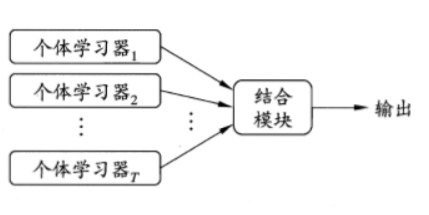
\includegraphics[width=0.8\linewidth]{5.PNG}
\end{center}
\centerline{集成学习示意图}
\subparagraph{boosting}Boosting是一族可将弱学习器提升为强学习器的算法。这一族算法的工作机制都是类似的:先从初始训练集训练出一个基学习器,再根据基学习器的表现对训练样本分布进行调整,使得先前基学习器做错的训练样本在后续受到更多关注,然后基于调整后的样本分布来训练下一个基学习器
\subparagraph{bagging}bagging算法以自助采样法(bootstrap sampling)为基础,从m个数据中\textbf{随机有放回地}取m个数据,约有近三分之一$(\ lim_ {m \to + \infty} \ (1 - \frac{1}{m})^m)$的样本不会被选中,将这些样本作为测试集,其余作为训练集。于是,我们可以采样出T个含m个训练样本的采样集,然后基于每个采样集训练出一个基学习器,再集成,这就是Bagging的基本流程。(参考西瓜书P173,P178)
\subparagraph{}自助法在数据集较小时很有用,并且能从初始数据集中产生多个不同的训练集,这对集成学习有很大的好处。 (西瓜书)

% Ensembling 部分 end



% lstm 部分 begin
\paragraph{\large 3.3.6 LSTM}.
\subparagraph{}LSTM网络非常适合基于时间序列数据进行分类,处理和预测,因为在时间序列中的重要事件之间可能存在未知持续时间的滞后。LSTM能够捕捉到这些滞后的关联。
\subparagraph{}LSTM单元有几种架构。通用架构由存储器单元,输入门,输出门和遗忘门组成。
\subparagraph{一些思考} 有论文对主流的深度学习模型进行了比较,指出LSTM在各类任务中表现优异,有十足的健壮性(robust),唯独在关键词识(keyphrase recognition)别例如情感识别中表现不如其他(当然也不差)。我觉得原因有在于句子的情感往往是鲜明的,反应在学习器的输出上的话这些输出值应当不是很连续的(趋向两级),LSTM捕捉的前后关联自然是没有精准定位情感词来的简单有效。(加上本身中立数据较多,使过拟合更为明显)


\begin{center} %插入的图片居中表示
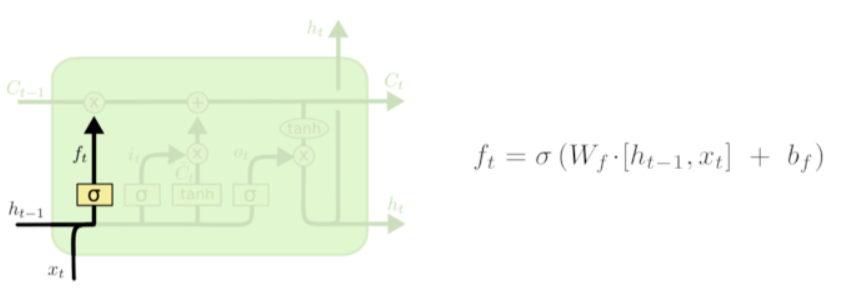
\includegraphics[width=0.8\linewidth]{1.PNG}
\end{center}
\centerline{遗忘门}
\subparagraph{}遗忘门取前一次的细胞状态C$_t$$_-$$_1$为输入,根据需要调权重输出C$_t$$_-$$_1$的一部分

\begin{center}
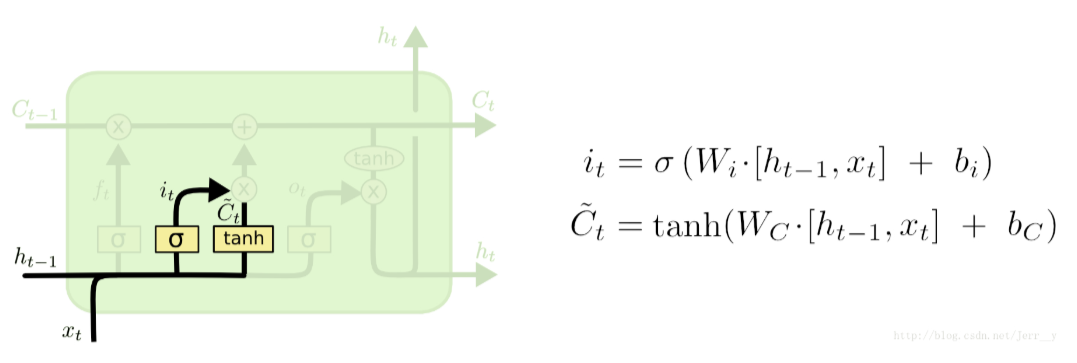
\includegraphics[width=0.8\linewidth]{2.PNG}
\end{center}
\centerline{输入门}
\subparagraph{}输入门决定让多少新的信息加入到细胞的状态中来

\begin{center}
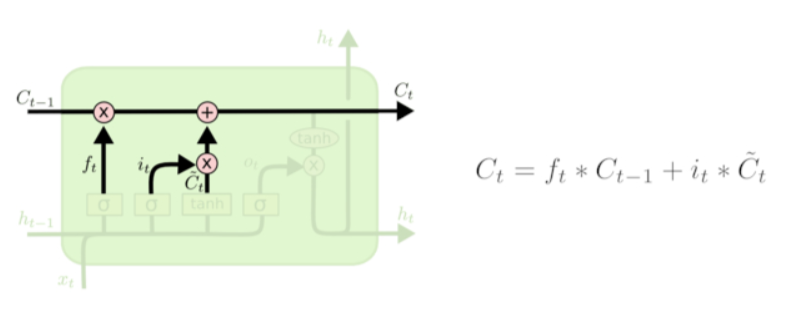
\includegraphics[width=0.8\linewidth]{3.PNG}
\end{center}
\centerline{更新后的细胞状态C$_t$}
\subparagraph{}输入门加上遗忘门就是新的细胞状态C$_t$

\begin{center}
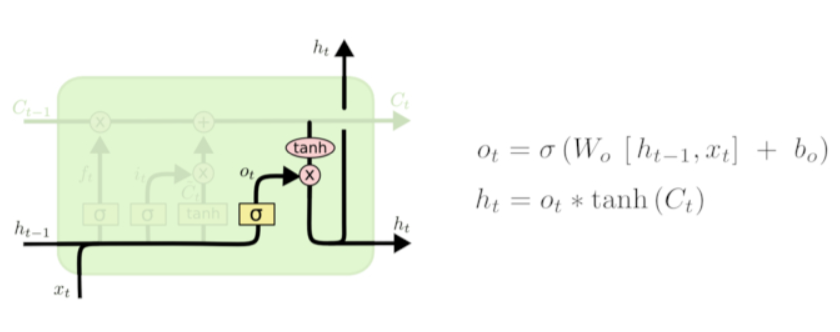
\includegraphics[width=0.8\linewidth]{4.PNG}
\end{center}
\centerline{输出门}
\subparagraph{}最后通过输出门,只输出我们想输出的部分,用于调节整个神经网络信息传递






\lstset{language=python}
\begin{lstlisting}
model = Sequential()
    model.add(Embedding(output_dim=vocab_dim,
                        input_dim=n_symbols,
                        mask_zero=True,
                        weights=[embedding_weights],
                        input_length=input_length))
    model.add(LSTM(output_dim=50, activation='tanh'))
    model.add(Dropout(0.8))
    model.add(Dense(3, activation='softmax'))
    model.add(Activation('softmax'))

    print('Compiling...')
    model.compile(loss='categorical_crossentropy',optimizer='adam',
                metrics=['accuracy'],sample_weight_mode='temporal')

    print("Train...")
    model.fit(x_train, y_train, batch_size=batch_size,
                                        epochs=n_epoch, verbose=1)

    print("Evaluate...")
    score = model.evaluate(x_test, y_test,batch_size=batch_size)
\end{lstlisting}
% lstm 部分 end

references:\\
wikipedia:LSTM\\
周志华:《机器学习》\\
Wenpeng Yin,Katharina Kann,Mo Yu, Hinrich Schutze.2017.Comparative Study of CNN and RNN for Natural Language Processing  \\



\end{document}
